\documentclass[12pt,preprint]{aastex}
%\documentclass{emulateapj}
\usepackage{amssymb,amsmath}
%\usepackage{caption}
%\DeclareCaptionLabelSeparator{dotemdash}{.--- }
%\captionsetup[figure]{labelformat=simple, labelsep=dotemdash}
%\usepackage{color,hyperref}
% hypertex insanity
%\definecolor{linkcolor}{rgb}{0,0,0.25}
%\hypersetup{
%  colorlinks=true,        % false: boxed links; true: colored links
%  linkcolor=linkcolor,    % color of internal links
%  citecolor=linkcolor,    % color of links to bibliography
%  filecolor=linkcolor,    % color of file links
%  urlcolor=linkcolor      % color of external links
%}
\newcounter{address}
\setcounter{address}{1}
%\usepackage{sidecap}
\setlength{\emergencystretch}{2em}%No overflowing references
\newcommand{\ie}{i.e.}
\newcommand{\etal}{et al.}
\newcommand{\dd}{\mathrm{d}}
\newcommand{\eg}{e.g.}
\newcommand{\eqnname}{equation}
\newcommand{\Eqnname}{Equation}
\newcommand{\equationname}{\eqnname}
\renewcommand{\tablename}{Table}
\renewcommand{\figurename}{Figure}
\newcommand{\figurenames}{\figurename~s}
\newcommand{\sectionname}{$\mathsection$}
\newcommand{\normal}{\ensuremath{\mathcal{N}}}
\newcommand{\flag}[1]{\texttt{\lowercase{#1}}}
\newcommand{\feh}{\ensuremath{[\mathrm{Fe/H}]}}
\newcommand{\afe}{\ensuremath{[\alpha\mathrm{/Fe}]}}
\newcommand{\logg}{log g}
\newcommand{\Ro}{\ensuremath{R_0}}

\renewcommand{\vec}[1]{\ensuremath{\mathbf{#1}}}
\newcommand{\unitvec}[1]{\ensuremath{\mathbf{\hat{#1}}}}
\newcommand{\vecx}{\ensuremath{\vec{x}}}
\newcommand{\vecv}{\ensuremath{\vec{v}}}
\newcommand{\vech}{\ensuremath{\vec{H}}}
\newcommand{\vecj}{\ensuremath{\vec{J}}}
\newcommand{\veco}{\ensuremath{\vec{\Omega}}}
\newcommand{\veca}{\ensuremath{\boldsymbol\theta}}
\newcommand{\df}{\ensuremath{f}}
\newcommand{\tdf}{\ensuremath{\mathrm{tDF}}}
\newcommand{\paramsdiff}{\ensuremath{\vec{p}_\Delta}}
\newcommand{\paramsdf}{\ensuremath{\vec{p}_{\mathrm{DF}}}}
\newcommand{\paramspot}{\ensuremath{\vec{p}_\Phi}}

\newcommand{\DF}{\df}
\newcommand{\dff}{\ensuremath{\mathbf{f}}}
\newcommand{\dex}{\ensuremath{\,\mathrm{dex}}}
\newcommand{\Gyr}{\ensuremath{\,\mathrm{Gyr}}}
\newcommand{\kpc}{\ensuremath{\,\mathrm{kpc}}}
\newcommand{\pc}{\ensuremath{\,\mathrm{pc}}}
\newcommand{\kms}{\ensuremath{\,\mathrm{km\ s}^{-1}}}
\newcommand{\msun}{\ensuremath{\,\mathrm{M}_{\odot}}}
\newcommand{\inv}{\ensuremath{^{-1}}}

\newcommand{\jr}{\ensuremath{J_R}}
\newcommand{\jphi}{\ensuremath{J_\phi}}
\newcommand{\jz}{\ensuremath{J_Z}}
\newcommand{\lz}{\ensuremath{L_Z}}
\newcommand{\Or}{\ensuremath{\Omega_R}}
\newcommand{\Ophi}{\ensuremath{\Omega_\phi}}
\newcommand{\Oz}{\ensuremath{\Omega_Z}}
\newcommand{\ar}{\ensuremath{\theta_R}}
\newcommand{\aphi}{\ensuremath{\theta_\phi}}
\newcommand{\az}{\ensuremath{\theta_Z}}

%\submitted{}

\begin{document}

\title{Dynamical modeling of tidal streams}
\author{Jo~Bovy\altaffilmark{1,2,3} \etal}
%  Hans-Walter~Rix\altaffilmark{4}}
\altaffiltext{\theaddress}{\label{IAS}\stepcounter{address} Institute
  for Advanced Study, Einstein Drive, Princeton, NJ 08540, USA}
\altaffiltext{\theaddress}{\label{Hubble}\stepcounter{address} Hubble
  fellow}
\altaffiltext{\theaddress}{\label{email}\stepcounter{address}
  Correspondence should be addressed to bovy@ias.edu~.}
%\altaffiltext{\theaddress}{\label{MPIA}\stepcounter{address}
%  Max-Planck-Institut f\"ur Astronomie, K\"onigstuhl 17, D-69117
%  Heidelberg, Germany}

\begin{abstract} 
  We present a generative, dynamical model for a tidal stream.
\end{abstract}

\keywords{
	Galaxy: fundamental parameters
	---
        Galaxy: kinematics and dynamics
        ---
	Galaxy: structure
}


\section{Introduction}


%BOVY: reference point


\section{Two equivalent generative models of tidal streams}\label{sec:method}

In this Section, we describe two mathematically equivalent generative
models for a tidal stream. The first is based on orbit integrations in
real (position-velocity) space: a tidal stream is generated from small
(phase-space) offsets between a star and a source\footnote{The word
  `progenitor' is typically used to indicate the actual parent body of
  a star in a tidal stream. For the dynamical model only a reference
  orbit from which the tidal stream can be thought of to originate is
  necessary; this reference orbit does \emph{not} have to coincide
  with the actual progenitor (this point is most clear in the
  description of the dynamics in action-angle coordinates). To avoid
  confusion between the hypothetical progenitor and the actual parent
  body, we refer to the reference orbit as the `source' rather than
  the `progenitor'.} that are evolved in time using orbit
integrations. The second method relies on the equivalent description
of this process in action-angle coordinates. While these two methods
are equivalent, the latter provides a conceptually simpler description
of the dynamical model and, when fitting a tidal stream, it allows for
fast marginalization over nuisance parameters. In particular, the
marginalization over the time at which a star was removed from the
source is analytic and the integration over possible source orbits can
be performed much faster (by avoiding orbit integrations of all
possible source orbits).

\subsection{Real-space model}\label{sec:realmethod}

The description of the stripping of a star from a satellite in real
(\vecx,\vecv) space assumes that at a time $\Delta t$ ago the star was
offset by a small amount ($\Delta \vecx,\Delta \vecv$) from the
position of the source $(\vecx^s,\vecv^s)(-\Delta t)$ at that
time. Then the star orbited under the influence of the same
gravitational potential $\Phi$ as the source until the present day
$(t=0)$, when it was observed: $(\vecx,\vecv)(t=0)$ = $\vech_{\Delta
  t}(\vecx^s(-\Delta t)+\Delta \vecx,\vecv^s(-\Delta t)+\Delta
\vecv)$, where $\vech$ denotes the Hamiltonian flow from $t=-\Delta t$
to $t=0$ (see \citealt{binneytremaine}); this is simply the orbit of
the star between these times. In phase-space this orbit can be
calculated by solving Hamilton's equations: $\dot{\vecx} = \vecv;
\dot{\vecv} = - \dd \Phi / \dd \vecx$. 

A generative model for the positions and velocities
($\vecx_i,\vecv_i$) of stars $i$ in a tidal stream is then fully
specified by: (a) the gravitational potential $\Phi$, (b) the current
phase-space position of the source $(\vecx_s,\vecv_s)(t=0)$, which can
be integrated backwards in time by reversing the Hamiltonian flow
defined by $\Phi$, (c) the time $\Delta t_i$ at which each star was
removed from the source, and (d) the distribution $f(\Delta
\vecx,\Delta \vecv|\paramsdiff)$, characterized by some parameters
$\paramsdiff$, of initial phase-space offsets from which the actual
offsets $(\Delta \vecx_i,\Delta \vecv_i)$ are drawn. In practice, $f$
can be taken to be a Gaussian, characterized by a width in position
$\sigma_x$ and in velocity $\sigma_v$, corresponding to the tidal
radius and escape velocity of the progenitor, respectively. However,
more complicated models for the initial phase-space distribution of
the debris can be used here as well (see discussion below). In the
case of a Gaussian $f$, the source can be thought of as the mean of
this Gaussian, with the additional requirement that this mean is an
orbit in the potential $\Phi$.

The probability for observing a star today at $(\vecx,\vecv)$ given
items (a) through (d) is then
\begin{align}\label{eq:realdft}
  p(\vecx_i,\vecv_i | \Phi,\vecx_s,\vecv_s,\Delta t_i,\paramsdiff) 
  & = p(\vecx_i(-\Delta t),\vecv_i(-\Delta t) | \Phi,\vecx_s,\vecv_s,\Delta t_i,\paramsdiff) \,,\nonumber\\
  & = p([\vecx_i-\vecx_s](-\Delta t),[\vecv_i-\vecv_s](-\Delta t) | \Phi,\vecx_s,\vecv_s,\Delta t_i,\paramsdiff) \,\nonumber\\
  & = p(\Delta\vecx_i(-\Delta t),\Delta\vecv_i(-\Delta t) | \Phi,\vecx_s,\vecv_s,\Delta t_i,\paramsdiff)\,,\\
  & = f(\Delta\vecx_i(-\Delta t),\Delta\vecv_i(-\Delta t) | \Phi,\vecx_s,\vecv_s,\Delta t_i,\paramsdiff)\, ,\nonumber
\end{align}
where the first equality holds because the Hamiltonian flow is unique
and conserves phase-space volume by Liousville's theorem and the
second one because the Jacobian of the transformation
$(\vecx_i,\vecv_i)(-\Delta t) \rightarrow (\vecx_i,\vecv_i)(-\Delta t)
- (\vecx_s,\vecv_s)(-\Delta t)$ is one. The final probability can be
evaluated using the parameters $\paramsdiff$ following (d).

The time $\Delta t_i$ at which a star was removed is unobservable and
the probability in \eqnname~(\ref{eq:realdft}) should therefore be
integrated over this time using a prior $p(\Delta t_i|\ldots)$, where
$\ldots$ indicates that this prior could depend on other factors such
as the potential and the progenitor orbit\footnote{For example, one
  could insist that stars are removed around pericenter passages. Note
  that this assumption would require the source orbit to be the actual
  progenitor orbit.}. For simplicity, we will assume a uniform prior
for the times $\Delta t$. The probability for a single star then becomes
\begin{align}\label{eq:realdf}
  p(\vecx_i,\vecv_i | \Phi,\vecx_s,\vecv_s,\paramsdiff) & = \int \dd
  \Delta t_i \,p(\vecx_i,\vecv_i | \Phi,\vecx_s,\vecv_s,\Delta t_i,
  \paramsdiff)\,.
\end{align}
If the progenitor's current phase-space position is unknown, then this
probability should be further marginalized over $(\vecx_s,\vecv_s)$;
for multiple stars, this marginalization is done after multiplying the
individual-star likelihoods in \eqnname~(\ref{eq:realdf}).

In practice, the likelihood in \eqnname~(\ref{eq:realdf}) can be
calculated as follows: for a given potential $\Phi$ and source
$(\vecx_s,\vecv_s)$, we (a) integrate the orbits of all stars
$(\vecx_i,\vecv_i)$ and (b) that of the source backward in time for
many Gyr and record the phase-space positions over time on a grid $j$
in $\Delta^j_i$; (c) we evaluate $f(\Delta \vecx_i,\Delta
\vecv_i)(\Delta t^j_i)$ for all stars $i$ and times $j$; (d) $f(\Delta
\vecx_i,\Delta \vecv_i)(\Delta t^j_i)$ is then summed over $j$ and the
logarithm of that is summed over $i$. The most computationally
expensive part of this calculation is the integration of the various
orbits. The evaluation of the likelihood for different parameters
\paramsdiff\ of $f$ can be efficiently computed by caching the orbit
integrations of (a) and (b); different source orbits
$(\vecx_s,\vecv_s)$ can also make use of the stored orbits in (a).

\subsection{Action-angle-space model}\label{sec:aamethod}

An alternative description of orbits in a gravitational potential
$\Phi$ is provided by the action-angle formalism (see
\citealt{binneytremaine} for an extensive description). The
Hamiltonian flow in the action-angle formalism is trivial: actions are
conserved and angles increase linearly with time. In
\appendixname~\ref{sec:aa} we summarize a method to calculate
action-angle coordinates from an orbit integration with little extra
work in any (static) potential for any kind of orbit. Therefore, it is
practical to use action-angle coordinates to describe the dynamical
model for a tidal stream in these coordinates and make use of the many
conceptual advantages provided by this formalism.

In the action-angle formalism, a star is removed from the source with
a small offset $(\Delta \vecj,\Delta \veca)(-\Delta t)$ from the
source's actions $\vecj_s$ and angles $\veca_s$ a time $\Delta t$ ago,
similar to the small offset $(\Delta \vecx,\Delta \vecv)(-\Delta t)$
in the real-space model. The offset in the actions corresponds to an
offset in the frequencies $\Delta \veco$; ultimately, this offset is
responsible for the spreading of the stream over long stretches on the
sky. Because both the source's angles and the star's angles increase
linearly with time, albeit at different frequencies, the difference in
the angles also increases linearly in time. Therefore at time $t=0$
the difference in angles is
\begin{equation}
\Delta \veca(t=0) = \Delta \veca(-\Delta t) + \Delta \veco \Delta t\,,
\end{equation}
while the difference in actions is constant
\begin{equation}
\Delta \vecj(t=0) = \Delta \vecj(-\Delta t)\,.
\end{equation}

With these preliminaries, we can write down a generative model for the
positions and velocities ($\vecx_i,\vecv_i$) of stars $i$ in a tidal
stream in the action-angle formalism by specifying: (a) the
gravitational potential $\Phi$, (b) the current action-angle
coordinates of the source $(\vecj_s,\veca_s)(t=0)$, (c) the time
$\Delta t_i$ at which each star was removed from the source, and (d)
the distribution $f(\Delta \vecj,\Delta \veca|\paramsdiff)$,
characterized by some parameters $\paramsdiff$, of initial phase-space
offsets from which the actual offsets $(\Delta \vecj_i,\Delta
\veca_i)$ are drawn. In practice, $f$ can again be taken to be a
Gaussian, although more general models could take the expected
`bowtie' structure of the action distribution into account
\citep{Eyre11a}. 

The probability for observing a star today at $(\vecx,\vecv)$ given
items (a) through (d) is then
\begin{align}\label{eq:aadft}
  p(\vecx_i,\vecv_i | \Phi,\vecj_s,\veca_s,\Delta t_i,\paramsdiff) 
  & = p(\vecj_i,\veca_i | \Phi,\vecj_s,\veca_s,\Delta t_i,\paramsdiff) \,,\nonumber\\
  & = p(\vecj_i-\vecj_s,\veca_i-\veca_s-\Delta \veco_i\Delta t_i | \Phi,\vecj_s,\veca_s,\Delta t_i,\paramsdiff) \,,\\
  & = f(\Delta \vecj_i,\Delta \veca_i(-\Delta t_i) | \Phi,\vecj_s,\veca_s,\Delta t_i,\paramsdiff) \,,\nonumber
\end{align}
where the first equality holds because the Jacobian of the
$(\vecx,\vecv)\rightarrow(\vecj,\veca)$ transformation is unity and
the second equality is a simple linear transformation. The final
probability can again be evaluated using the parameters
\paramsdiff\ following (d).

As in the real-space formalism, we should integrate
\eqnname~(\ref{eq:aadft}) over the time $\Delta t_i$ at which the star
is removed from the source (cf.~\eqnname~[\ref{eq:realdf}]):
\begin{equation}\label{eq:aadf}
  p(\vecx_i,\vecv_i | \Phi,\vecj_s,\veca_s,\paramsdiff) = \int \dd
  \Delta t_i\, f(\Delta \vecj_i,\Delta \veca_i(-\Delta t_i) |
  \Phi,\vecj_s,\veca_s,\Delta t_i,\paramsdiff) \,.
\end{equation}
Without further assumptions the action-angle formalism proceeds in the
same way as the real-space formalism, evaluating
\eqnname~(\ref{eq:aadft}) for a grid $j$ of times $\Delta t_i^j$ and
summing $f(\Delta \vecj_i,\Delta \veca_i(-\Delta t^j_i) |
\Phi,\vecj_s,\veca_s,\Delta t_i,\paramsdiff)$ over $j$.

Even without further assumptions about the shape of $f(\Delta
\vecj,\Delta \veca|\paramsdiff)$, the action-angle formalism already
allows for a simplification over the real-space method. Because the
source orbit is specified in action-angle coordinates, it can be
changed \emph{without} expensive orbit integrations of all possible
source orbits. As the source's current phase-space position is a
six-dimensional parameter, this is a major simplification of the
dynamical model when the source orbit is unknown. Note that this
simplification does require us to be able to compute $\veco(\vecj)$,
to calculate the new source frequencies $\veco_s$ when changing the
source actions $\vecj_s$. This mapping can be constructed using a
small number of (action,frequency) calculations covering the range of
possible source actions.

We can simplify \eqnname~(\ref{eq:aadf}) by assuming (a) that
$f(\Delta \vecj,\Delta \veca|\paramsdiff)$ is separable into
$f_{\veca}(\Delta \veca|\paramsdiff)\,f_{\vecj}(\Delta
\vecj|\paramsdiff)$ and (b) that the distribution $f_{\veca}(\Delta
\veca|\paramsdiff)$ is Gaussian. In what follows, we will assume that
this Gaussian is isotropic with dispersion $\sigma_\theta$, but all of
the results are the same after appropriate diagonalization and
rescaling of the angles for more general covariance matrices. In this
case, \eqnname~(\ref{eq:aadf}) can be written as
\begin{equation}
\begin{split}
  p(\vecx_i,\vecv_i & | \Phi,\vecj_s,\veca_s,\paramsdiff) 
   = \\
   & f_{\vecj}(\Delta \vecj_i|\paramsdiff) \int \dd \Delta t_i\,
  \frac{1}{(2\,\pi)^{3/2}\,\sigma_\theta^3}\,\exp\left(-\frac{1}{2\,\sigma_\theta^2}\left[\sum_{R,\phi,Z}\left(\Delta \veca_i-\Delta \veco_i\Delta t_i\right)^2\right]\right)\,,
\end{split}
\end{equation}
where the sum in the argument of the exponential is over the three
components of $\Delta \veca_i$ and $\Delta \veco_i$. This integral can
be done analytically, resulting in
\begin{equation}\label{eq:aadfsimple}
\begin{split}
  p(\vecx_i,\vecv_i & | \Phi,\vecj_s,\veca_s,\paramsdiff) 
   = \\
   & f_{\vecj}(\Delta \vecj_i|\paramsdiff) \,  \frac{1}{2\,\pi\,\sigma_\theta^2\,\sqrt{\sum_{R,\phi,Z}\Delta \veco_i^2}}\,\exp\left(-\frac{1}{2\,\sigma_\theta^2}\left[\sum_{R,\phi,Z}\Delta \veca^2_i-\frac{\left(\sum_{R,\phi,Z} \Delta \veco_i\Delta \veca_i\right)^2}{\sum_{R,\phi,Z}\Delta \veco_i^2}\right]\right)\,.
\end{split}
\end{equation}
In this expression, $\Delta X^2 \equiv (X_1-X_2)^2$. The expression in
square brackets is positive by using the Cauchy-Schwarz inequality.

The quantity in the square brackets in \eqnname~(\ref{eq:aadfsimple})
expresses the fact that the present-day difference in angles between a
star in a tidal stream and the source must be linearly related by a
scalar (the time since the removal of the star) to the difference in
frequencies, within a tolerance set by the width of the distribution
of initial angle differences ($\sigma_\theta$). The ratio
$\sum_{R,\phi,Z} \Delta \veco_i\Delta \veca_i/\sum_{R,\phi,Z}\Delta
\veco_i^2$ is the best-guess for $\Delta t_i$ when performing a linear
regression between $\Delta \veca_i$ and $\Delta \veco_i$. The
expression in square brackets is minimized when the correlation
between $\Delta \veca_i$ and $\Delta \veco_i$ is the largest, \ie,
when a single time difference $\Delta t_i$ explains all three of the
angle differences.

The discussion so far has been entirely general and applies to any
sort of stellar debris that originates from a single orbit, without
necessarily generating a one-dimensional structure. In most
observations of tidal streams, however, they appear as one-dimensional
objects rather than the six-dimensional objects that we have
considered so far. The reason for this is both physical and
observational: (a) narrow tidal streams form because a star separates
from the progenitor over time mostly along a single direction in
angle-space: the Hessian matrix of the Hamiltonian, $\partial^2 H /
\partial \vecj \partial \vecj$, has a single large eigenvalue, which
determines the direction along which the stream is disrupted in
angle-space (because $\partial \veco / \partial \vecj$ is equal to the
Hessian); (b) because many tidal streams are dynamically cold with
velocity dispersions $\lesssim10\kms$, observations are unable to
resolve the angle differences along the two eigenvectors of the
Hessian corresponding to the two smallest eigenvalues or the spread in
actions among stream members. If the latter can be resolved, the
stream is four-dimensional. In what follows we will be mainly
concerned with the stream only spreading along a single direction in
angle space.

If the stream is one-dimensional in angle space then the time since
the removal from the progenitor becomes unobservable if the progenitor
orbit is unknown: above, determining the time depended on explaining
the three-dimensional angle difference $\Delta \veca$ with the
three-dimensional frequency difference $\Delta \veco$ using a single
time difference; if two of the angle and frequency differences are
unable to be resolved, then the frequency difference and the time
difference become degenerate (aka, you can draw a straight line
connecting any two points). To make use of this fact to simplify the
dynamical model, we write the frequency difference as
\begin{equation}
  \Delta \veco = \Delta \Omega_1\,\unitvec{e}_1\,,
\end{equation}
where $\unitvec{e}_1$ is a unit vector. Then we write the angle
difference $\Delta \veca$ 
\begin{equation}
  \Delta \veca = \Delta \theta_1\,\unitvec{e}_1 + \Delta \veca_\perp\,\unitvec{e}_1^\perp\,,
\end{equation}
where$\unitvec{e}_1^\perp$ is the orthogonal complement of
$\unitvec{e}_1$ (the two directions perpendicular to $\unitvec{e}_1$)
and $\Delta \veca_\perp$ are the components of $\Delta \veca$ in that
direction. We can then write \eqnname~(\ref{eq:aadfsimple}) as
\begin{equation}\label{eq:aadfsimpler}
\begin{split}
  p(\vecx_i,\vecv_i & | \Phi,\vecj_s,\veca_s,\paramsdiff) 
   = \\
   & f_{\vecj}(\Delta \vecj_i|\paramsdiff) \,  \frac{1}{2\,\pi\,\sigma_\theta^2\,\sqrt{\sum_{R,\phi,Z}\Delta \veco_i^2}}\,\exp\left(-\frac{|\Delta\veca_{i,\perp}|^2}{2\,\sigma_\theta^2}\right)\,.
\end{split}
\end{equation}
\Eqnname~(\ref{eq:aadfsimpler}) is equivalent to
\eqnname~(\ref{eq:aadfsimple}), but it expresses the dynamical model
in a slightly different way. Whereas the angle part of
\eqnname~(\ref{eq:aadfsimple}) allows the correct potential and
progenitor to be inferred by asking whether a single time difference
explains the three angle differences given the three frequencies,
\eqnname~(\ref{eq:aadfsimpler}) `rewinds' the star's orbit along the
direction of $\Delta \veco$ and asks whether the angle difference
perpendicular to $\Delta \veco$ is consistent with the initial angle
spread (because it has not evolved since the removal of the star). In
re-writing this, we have not yet used the approximation that the
stream only forms along a single direction in $\Delta \veco$.





This view of the dynamics of the stream in action-angle coordinates
also shows that the orbit of the source does not have to coincide with
that of the actual progenitor. 

The probability in \eqnname~(\ref{eq:aadfsimple}) incorporates and
elucidates commonly used methods for fitting tidal streams. On the one
hand are approaches that search to minimize the spread in energy,
integrals of the motion, or actions (\eg,
\citealt{Binney08a,Penarrubia12a}, Sanderson \etal, 2013, in
preparation). These approaches ignore the correlations between actions
and angles in the stream (the exponential in
\eqnname~(\ref{eq:aadfsimple}), which describes this correlation
through the frequencies) and only use $f_{\vecj}(\Delta
\vecj_i|\paramsdiff)$; finding the gravitational potential that
minimizes the spread in actions optimizes $f_{\vecj}(\Delta
\vecj_i|\paramsdiff)$. Recently, a method was proposed that only uses
the correlation between the actions and the angles, expressed by the
exponential in \eqnname~(\ref{eq:aadfsimple}) \citep{Sanders13a}; this
method does not use the fact that the spread in actions in a tidal
stream is small (expressed by $f_{\vecj}(\Delta
\vecj_i|\paramsdiff)$).


%BOVY: reference point

\acknowledgements It is a pleasure to thank \dots for helpful comments
and assistance. J.B. was supported by NASA through Hubble Fellowship
grant HST-HF-51285.01 from the Space Telescope Science Institute,
which is operated by the Association of Universities for Research in
Astronomy, Incorporated, under NASA contract NAS5-26555. J.B.
%and H.-W.R  (BOVY: ALSO ACKNOWLEDGE WITHOUT S)
acknowledges support from SFB 881 (A3) funded by the German
Research Foundation DFG.


\appendix

\section{An efficient, general method for calculating action-angle coordinates using orbit integration}\label{sec:aa}


\section{Dynamical modeling of two-star streams}\label{sec:twostar}

%BOVY: reference point

\begin{thebibliography}{}

\bibitem[{{Binney} \& {Tremaine}(2008)}]{binneytremaine}
  Binney,~J. \& Tremaine,~S. 2008, Galactic Dynamics: Second Edition
\bibitem[Binney(2008)]{Binney08a}
  Binney,~J. 2008, \mnras, 386, L47
\bibitem[Eyre \& Binney(2011)]{Eyre11a}
  Eyre,~A. \& Binney,~J. 2011, \mnras, 413, 1852
\bibitem[Pe{\~n}arrubia \etal(2012)]{Penarrubia12a}
  Pe{\~n}arrubia, J., Koposov,~S.~E., \& Walker,~M.~G. 2012, \apj, 760, 2
\bibitem[Sanders \& Binney(2013)]{Sanders13a}
  Sanders,~J. \& Binney,~J. 2013, \mnras, 433, 1826
\end{thebibliography}


\begin{figure}[t!]
  \includegraphics[width=0.5\textwidth,clip=]{gd1_evol_xz.ps}
  \caption{}\label{fig:gd1_xy}
%python plot_stream.py ../tex/gd1_evol_xz.ps
\end{figure}

\begin{figure}[t!]
  \includegraphics[width=\textwidth,clip=]{gd1_evol_lb.ps}
  \includegraphics[width=\textwidth,clip=]{gd1_evol_ld.ps}
  \caption{}\label{fig:gd1_xy}
%python plot_stream.py ../tex/gd1_evol_lb.ps
%python plot_stream.py ../tex/gd1_evol_ld.ps
\end{figure}

\begin{figure}[t!]
  \includegraphics[width=0.32\textwidth,clip=]{gd1_evol_aajrjz.ps}
  \includegraphics[width=0.32\textwidth,clip=]{gd1_evol_aaoroz.ps}
  \includegraphics[width=0.32\textwidth,clip=]{gd1_evol_aaaraz.ps}\\
  \includegraphics[width=0.32\textwidth,clip=]{gd1_evol_aajrjp.ps}
  \includegraphics[width=0.32\textwidth,clip=]{gd1_evol_aaorop.ps}
  \includegraphics[width=0.32\textwidth,clip=]{gd1_evol_aaarap.ps}
  \caption{}\label{fig:gd1_xy}
%python plot_stream.py ../tex/gd1_evol_aajrjz.ps
%python plot_stream.py ../tex/gd1_evol_aaoroz.ps
%python plot_stream.py ../tex/gd1_evol_aaaraz.ps
%python plot_stream.py ../tex/gd1_evol_aajrjp.ps
%python plot_stream.py ../tex/gd1_evol_aaorop.ps
%python plot_stream.py ../tex/gd1_evol_aaarap.ps
\end{figure}

\end{document}
